\documentclass[11pt, a4paper]{article}

\usepackage[utf8]{inputenc}
\usepackage{fullpage}
\usepackage[parfill]{parskip} % Empty line instead of indentation
\usepackage{graphicx}
\graphicspath{ {images/} }
\usepackage{listings}
\usepackage{mathtools}
\usepackage{amssymb}
\usepackage{eurosym} %Euro symbol
%\usepackage[ngerman]{babel}
\usepackage{cancel} % Cancel fractions
\usepackage{units}
\usepackage{xcolor}
\usepackage{setspace}

\newcommand\braces[1]{\left(#1\right)}
\newcommand\brackets[1]{\left[#1\right]}
\renewcommand{\vec}[1]{\underline{#1}}
\newcommand{\mat}[1]{\underline{\underline{#1}}}
\newcommand{\abs}[1]{\left\lvert#1\right\rvert}
\newcommand{\norm}[1]{\left\lVert#1\right\rVert}
\newcommand\tr[1]{\mathrm{tr}\br{#1}}
\newcommand\average[1]{\left\langle#1\right\rangle}
\newcommand{\acos}[1]{\mathrm{acos}\braces{#1}}
\newcommand{\asin}[1]{\mathrm{asin}\braces{#1}}
\newcommand{\intend}[1][]{\ \mathrm{d}#1}
\newcommand{\derivative}[2][]{\ \frac{\mathrm{d}#1}{\mathrm{d}#2}} %\derivative[a]{b}
\newcommand\expectedValue[1]{\mathbb{E}\braces{#1}}
\newcommand\variance[1]{\mathbb{V}\braces{#1}}
\newcommand\setequal{\overset{!}{=}}
\newcommand{\gerquote}[1]{\glqq#1\grqq}
\definecolor{AI-BLUE}{rgb}{0,0.57,0.87}

\onehalfspacing
\setlength\parindent{0pt}
\allowdisplaybreaks

\title{TITLE}
\author{AUTHOR}
\date{\today}

\makeatletter
    \setlength\@fptop{0\p@}
\makeatother

\begin{document}
\thispagestyle{empty}

\begin{titlepage}
    \begin{center}
    \vphantom{0cm}
    \huge \textbf{Hardening artificial neural networks against specifically constructed adversarial input data} \\
    \vspace{4cm}
    %\LARGE \textbf{Report}\\
    \normalsize
    Written Master Thesis Report \\
    for the Masters Program of \textcolor{AI-BLUE}{[Applied Computer Science]}\\
    at the Ruhr-University Bochum\\
    in the Summer Term 2016\\
    \vspace{4cm}
    %\normalsize
    \textbf{Submitted by}\\
    B. Sc. Christian Andreas Mielers (108 011 204 956)\\
    \vspace{1cm}
    \today \\
    \vspace{1cm}
    \textbf{Supervisors} \\
    PD Dr. Rolf P. Würtz \\
    M. Sc. Andreas Nilkens
    \end{center}
\end{titlepage}

\newpage
\pagenumbering{arabic}
\setcounter{page}{2}

\tableofcontents

\newpage
\section{Introduction}
As the problems people try to solve with the aid of computers become more and more complex, their ability to write software that can keep up with those aspirations does not follow suit. Solving more complex problems with software does not only incur the cost of finding viable solutions and formalizing them in computer code, but also the cost of integrating all the necessary components, organizing their interactions, ensuring they use common resources in a well-defined manner, and testing all of the above. These tasks grow essentially super-linearly in difficulty, and can thus quickly become harder than the problem that the system was initially meant to solve.

One way out of this dilemma that people turn to increasingly often is the usage of machine learning techniques. The goal of machine learning is to free people from the burden of finding and programming a solution. In order to do so, a \emph{model} is defined which embodies the structure of a possible solution on a highly abstract level. However, such a model as potentially a myriad of \emph{parameters}, and no knowledge of reasonable values for those parameters can be assumed. What gives machine learning its name and makes it feasible despite the many unknown parameters is the learning method. This is a method to find a working configuration of parameters based on \emph{training data}. In \emph{supervised learning}, the algorithm that performs the learning is provided numerous pairs of an exemplary input and the corresponding desired output that the model should deliver. From these pairs, it extracts, or \emph{learns}, the relationship between input and output data, and codifies it in the model's parameters. In this manner, the need for a handcrafted solution is eliminated. The downside to this approach is that learning algorithms usually require a copious amount of training data to find good parameters. However, this drawback is increasingly often offset by the reduced software complexity, since machine learning models usually have a well-defined theoretical foundation with ready-made software available.
% TODO write something about verification with test data?

% TODO substantiate claim that ANNs are among the top machine learning models
Among some of the most momentous machine learning models are \emph{artificial neural networks (ANNs)}. They are inspired by discoveries from the field of neural biology and incorporate them into models that, on a very abstract level, resemble brain structures on the detail level of individual neurons. The workings of these  neuron are greatly simplified, but in this way they can be easily connected in large bulks, empowering the resulting network to solve difficult tasks with impressive precision. ANNs are mainly used to two types of tasks: \emph{classification} and \emph{regression}. While the latter is concerned with learning a function $f: X \rightarrow Y$ that maps input data to the desired output values, it is the former that will be of interest within the scope of this thesis. Classification instead aims to assign each input to one category out of a predefined set of categories. The data used to train the network is structured accordingly: it consists of the input data and a \emph{label} that denotes its class.
% TODO note that learner for neural networks is "gradient descent"?

% TODO illustrate image classification
One area where neural networks are particularly successful is \emph{image classification}, the task of classifying an object by from a digital photo of it. A big part of the success here can be attributed to a special variant of ANNs, called \emph{Convolutional Neural Networks (CNNs)}. These networks focus on local features in the input by applying \emph{filters} in a convolution operation, thereby curtailing redundancies in the free parameters. Combined with the focus on local features, this efficient use of free parameters allows for much larger and thus more powerful networks.

% TODO illustrate training and test steps with an image
When training a neural network for an image classification task, one desires a CNN to not only classify the images used for training correctly, but to infer and learn the fundamental characteristics of each class. Only then will the network be able to \emph{generalize} its classification capabilities to the previously unseen images it will encounter in productive use. To gauge a network's ability to generalize, another data set, called the \emph{test set} is usually withheld while training the model. The experimenter can then evaluate the performance on this set outside of training, thus obtaining an estimator for field performance of the model.

In the past, ANNs in general and CNNs in particular have shown convincing results not only on training data but also test data. However, recent discoveries have indicated that the generalization capability of most neural networks is not as strong as one might guess from test set performance. While networks certainly can classify unseen input with high reliability, it is possible to find minute transformations of correctly classified test data, on which the network will predict another class with high confidence. The changes that need to be applied for this to work are miniscule and undetectable to the human eye. The resulting images are called \emph{adversarial examples (AEs)}.

In the initial publication a rather complex method for creating those images was presented. A major impediment of this method was the excessive computational power and time required to produce AEs. Fortunately, a follow-up paper greatly improved the feasibility of this process by introducing a gradient-based procedure for generating AEs. In that manner a considerable amount of AEs can be generated in a reasonable time frame, enough to allow for reasonable quantitative analysis of the AE's properties. Therefore, this thesis will look at various statistics of larger groups of AEs, including their spectra and the ways these spectra differ from those of unadulterated images. Regarding the spectra, we will also look at the distribution of values with regards to the frequency and orientation.

Furthermore, the process of generating adversarial examples can be inspected on a considerably larger scale. Plots for the network confidence on images in the process of being turned into AEs will provide insights on the process with regards to iteration count, and serve as the foundation for attempts to predict whether an image can be successfully made adversarial. Data on the success rate of converting images to adversarial examples will be presented, both per original and adversarial class as well as overall figures.

The aforementioned results will be obtained with multiple data sets and various network layouts and parameter configurations. The latter will also allow for inspection of the impact of parameter choice on various statistics.

% History
%% What is a neural network
%% Strengths
%% Industry applications
%% The problem with adversarial examples
%% What this thesis is about
% Future prospects

\newpage
\section{Artificial Neural Networks}
In the area of machine learning, artificial neural networks are some of the most widely studied models. They stem from insights into the workings of real, biological brains in the field of neural biology. Here, the individual neuron is used as the fundamental unit of computation. A schematic version of the biological variant is shown in figure \ref{fig:biological-neuron-schematic}.

\begin{figure}[htp]
	\centering
	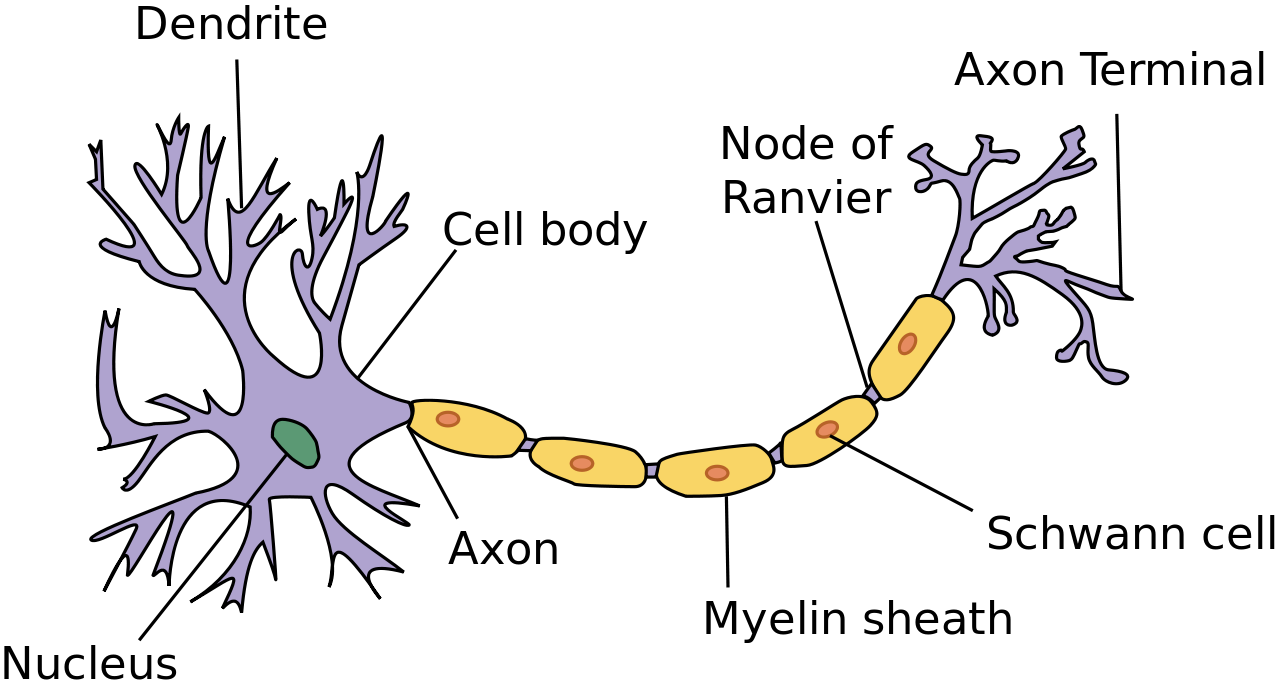
\includegraphics[width=0.5\textwidth]{images/biological_neuron.png}
	\caption{Schematic of a biological neuron, taken from \cite{biological-neuron-schematic}}
	\label{fig:biological-neuron-schematic}
\end{figure}

% TODO be a bit more precise here with the chemistry
A neuron receives incoming electrical pulses, called \emph{action potentials}, from the axons of other neurons via its dendrites. A connection between an axon and a dendrite is called a \emph{synapse}. These synapses can vary in strength, so the intensity of the received pulse is modulated by the synaptic connectivity. Multiple action potentials may arrive in the soma, the cell body of a neuron, in quick succession, causing the membrane potential of the soma to increase. If enough action potentials arrive within a short time via strong synapses, this may cause the cell in question to initiate an action potential which traverses along its axon. This can be considered to be a decision of the sell to pass the message on to other cells.

An artificial neuron as used in an ANN mimics this process, but in a greatly simplified form. All action potential rates are represented by real numbers\footnote{Floating point numbers in a computer system}. A visual representation is provided in figure \ref{fig:artificial-neuron-schematic}.


\begin{figure}[htp]
	\centering
	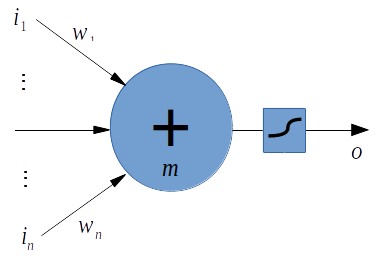
\includegraphics[width=0.45\textwidth]{images/artificial_neuron.png}
	\caption{Schematic of an artificial neuron}
	\label{fig:artificial-neuron-schematic}
\end{figure}

The first thing to note is that the input to the neuron is now formalized as a vector $\vec{i}$ with components $i_1 \dots i_n$, where $n$ represents the number of inputs that influence this neuron. Each input value $i_j$ is multiplied with a \emph{weight}, denoted by $w_j$. This weight can be thought of as an abstraction of the synaptic strength between two neurons. Then, all of these input-weight pairs are summed up to realize the counterpart to the membrane potential, labeled $m$. To form the neuron's output $o$, one last step is neccessary. In biological neurons, the rate of outgoing spikes of a neuron is not linear in the incomming spikes. Thus, a nonlinear \emph{activation function} is applied to the membrane potential $m$, symbolized by the sigmoidally shaped line in the rectangular box in figure \ref{fig:artificial-neuron-schematic}. If that activation function is called $\sigma$, the mathematical operation performed by a single neuron can be summarized according to equations \eqref{eq:neuron-math-membrane-potential} and \eqref{eq:neuron-math-activation-function}.

\begin{align}
	m &= \sum_{i=1}^n w_n \cdot i_n = \vec{w}^T \vec{i} \label{eq:neuron-math-membrane-potential} \\
	o &= \sigma \braces{m} \label{eq:neuron-math-activation-function}
\end{align}



% TODO will it only become especially important in chapter 3, or also in other places?
Take note of the fact that the very first step performed on the input is essentially an inner product. This will become important later on, especially in chapter \ref{sec:adversarial-examples}. Several activation functions are possible. A plot of 3 common choices is given in figure \ref{fig:activation-functions}.

\begin{figure}[htp]
	\centering
	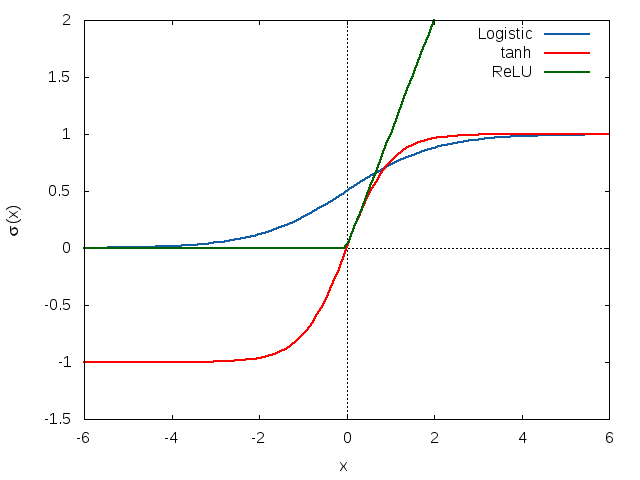
\includegraphics[width=0.6\textwidth]{images/activation_functions.png}
	\caption{Logistic sigmoidal, hyperbolic tangent and ReLU activation functions}
	\label{fig:activation-functions}
\end{figure}

Out of these, the easiest to justify is the logistic sigmoid. If the output is to represent the neuron's firing rate, it must not become negative, and it must saturate because of the refractory period required by biological cells. Under these conditions, the logistic function is a simple continuous choice. The hyperbolic tangent is a linearly transformed version of this. While its negative range may be harder to interpret biologically, the option to output negative values may relieve the trainable parameters of a network of some demand for computational power, thus facilitating training. Despite being non-continuous and having no upper bound, the ReLU is the most popular activation function according to \cite{deep-learning-2015}. The networks utilized in this thesis mostly make use of the $\tanh$ and ReLU activation functions.

Since a single neuron as described above consists only of an inner product and a one-dimensional non-linearity, its computational power is limited. Artificial neural networks rely on thousands of neurons to perform their tasks. This gives rise to the question of how to connect all those neurons. Conceptually, one could link them up in such a way that a neuron that receives input from another neuron while at the same time delivering input to that same neuron (either directly or via proxy neurons), forming a cycle. This is sometimes done in practice and is called a \emph{Recurrent Neural Network (RNN)}, but is out of scope for this thesis. Instead, neurons will be organized in \emph{layers}, as shown in figure \ref{fig:neural-nework-structure}. %TODO

\begin{figure}[htp]
\centering
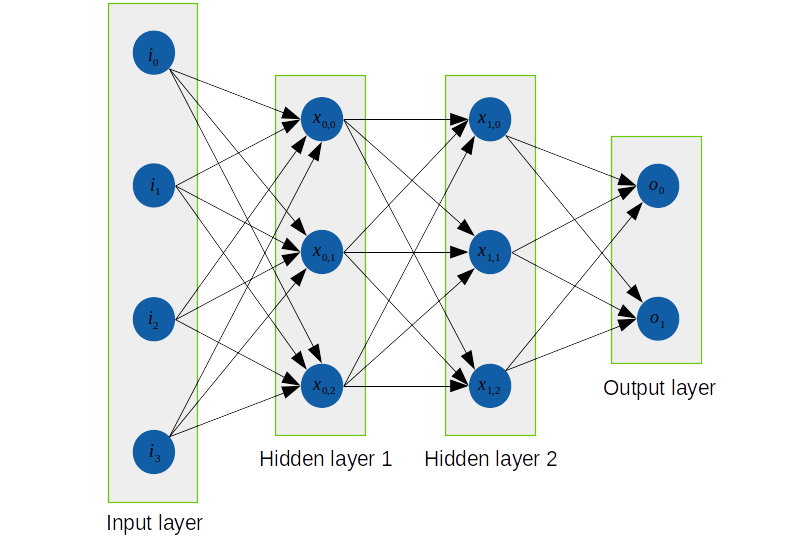
\includegraphics[width=\textwidth]{images/network_layout.png}
\caption{Structure of neuron arrangement in an ANN}
\label{fig:neural-nework-structure}
\end{figure}

% TODO back up claim that input layer is called "first and "lowest" layer
% TODO use top-down image instead of left-right. Requires to reformulate the text a bit.
Here, each layer contains numerous neurons, none of which share a connection. This means that there is no interaction within a layer and thus it seems reasonable to inspect the actions of a network in a layer-by-layer fashion. The layer on the left is often called the "first" or "lowest" layer, and it is the spot where the input data is feed into the network. Therefore, its neurons deviate from the description given in figure \ref{fig:artificial-neuron-schematic} and equations \eqref{eq:neuron-math-membrane-potential} and \eqref{eq:neuron-math-activation-function}. No computation takes place here, the data is taken as-is and used as input for the layer above.

% TODO be more specific about the universal approximation theoren
% TODO describe layers as homeomorphisms according to http://colah.github.io/posts/2014-03-NN-Manifolds-Topology/
In the figure the layer above the input contains 3 neurons and is named "Hidden layer 1". Hidden layers are those that are neither input nor output and thus do not communicate with any system outside the network. Note that each neuron here has two indices: The first one designates the layer affiliation and the second one identifies the individual neuron. The first hidden layer is followed by a second one. A neural network can conceptually have an unlimited amount of hidden layers, but at least one is necessary to satisfy the \emph{universal approximation theorem} which attests that for every function, there exists a neural network that can approximate said function to a arbitrary but fixed accuracy\footnote{However, this is of limited practical use, since the theorem makes no statement about the required number of neurons, or how to set the weights.}.

A further notational simplification can be made at this point. Equation \eqref{eq:neuron-math-membrane-potential} described the operation of a single neuron as an inner product. If we treat the output of \emph{Hidden layer 1} as a vector $\vec{x_0}$ and the output of \emph{Hidden layer 2} as another vector $\vec{x_1}$, the entire operation of the second hidden layer can be described by a matrix-vector product according to equations \eqref{eq:layer-math-membrane-potential} and \eqref{eq:layer-math-activation-function}.

\begin{align}
	\vec{m_1} &= \mat{W_{1}} \, \vec{x_0} \label{eq:layer-math-membrane-potential} \\
	\vec{o_1} &= \sigma \braces{\vec{m_1}} \label{eq:layer-math-activation-function}
\end{align}

where $\sigma \braces{\vec{m_1}}$ indicates the element-wise application of the activation function to the membrane potentials. If the weight vectors used in equation \eqref{eq:neuron-math-membrane-potential} are used as row vectors of $\mat{W_1}$, then this is an equivalent description on a higher level of abstraction. This can of course be done analogously for the other layers of the network.

Beyond biological plausibility, this formalism provides another justification for using activation functions at all. If they were not part of a neural network model, each layer would solely perform a matrix-vector product, which, due to their linear properties, could be collapsed into a single matrix-vector product, greatly reducing the model's capacity to describe complex relations between input data and output data.

% TODO source for softmax function
The last layer generates the output of the network. It too can in part be described as a matrix-vector product. It may also share the same activation function as other layers, in which case its functionality is mostly identical with hidden layers. However, this is sometimes inappropriate. In regression, for instance, the range of the function to be learned may go far into the negative range, well below $-1$. None of the activation functions shown in figure \ref{fig:activation-functions} are capable of modelling this. Similarly, in classification, it might be desirable for the output to represent the probabilities of an input belonging to each of the classes. While all of the discussed activation functions include the range $[0-1]$, thereby making such a representation possible, other activation functions specifically suited for output layers, like the \emph{softmax function}, can force those properties.

% TODO Deep dream
% TODO Akin to layered processing in vision
% TODO Back up the claim that first layer is usually feature extractor / corner detector.
The relatively recent machine learning trend going by the name of \emph{deep learning} builds extensively on this layered architecture of neural networks. Specifically, \emph{deep} neural networks use many more hidden layers than just 1, in contrast to the preceding networks, which were ex post named \emph{shallow} networks. The central hypothesis of this approach is that the various layers of a network will learn to perform distinct, hierarchically structured functions. Typically, the first layer (or first few layers) are expected to become low-level feature extractors, providing basic information for the higher layers. In vision tasks, for example, one can often observe that the lowest layer works as a corner detector, because the geometry within an image often contains the most important information. The following layers the hopefully extract features with an increasing level of abstraction, e.g. combining corners to edges and more complex shapes and contours. The last layer is tasked with making the final decision regarding the input object's class, using the presence of those high-level features as the basis for its choice.

% TODO some networks make use of this? Sure its not all of them?
% TODO glorot formula
% TODO caffe does glorot initialization slightly differently
One question that has not been addressed yet is how to actually set the weights. Under normal circumstances there is no closed form solution to compute the optimal parameters for a model. Thus, an training process that starts with a random set of weights and then iteratively improves on them is used. To accomplish random initialization, values for all weights are drawn from one of various distributions. Common choices are uniform, normal distributions. In 2010, a more sophisticated method has been proposed in \cite{glorot-understanding-deep-nn-training}. It still relies on a uniform initialization, but the limits are set for each layer individually, in order to retain the variance the data as it flows through the layers of the network. Some networks in this thesis make use of this advanced initialization.

In order to improve the thusly initialized weights, it is first necessary to define a way to quantify how well (or poorly) a given set of parameters performs. To this end, an \emph{loss function} (also called \emph{objective function} or \emph{error function}) is used, which combines the predictions of a network with the training labels to provide an estimate of its performance. In other words, it is a function that maps labeled input data and the parameters to a scalar value. A common loss function is the \emph{Mean Squared Error (MSE)} given in equation \eqref{eq:mse}, where $N$ is the number of data points and $\vec{\hat Y}$ and $\vec{Y}$ are vectors containing the prediction and true label, respectively. In multinomial classification tasks, the \emph{cross entropy} loss given in equation \eqref{eq:cross-entropy-loss} \cite{caffe-cross-entropy} is a good choice if the predictions for all classes are to be interpreted as probabilities (meaning they are required to add up to 1). Here, $\vec{\hat Y}$ is a matrix containing all predicted class probabilities for all $N$ data points and $\vec{Y}$ is a vector indicating the true class.

% TODO source for MSE
% TODO make this more readable
\begin{align}
	\text{MSE} &= \frac{1}{N} \sum_{i=1}^N \braces{\vec{\hat Y}_i - \vec{Y}_i}^2 \label{eq:mse} \\
	\text{Cross entropy} &= \frac{-1}{N} \sum_{i=1}^N \log{\braces{\mat{\hat Y}_{i, \vec{Y}_i}}} \label{eq:cross-entropy-loss}
\end{align}

The goal of neural network training is usually to minimize the loss function (although it could be maximization depending on the formulation of the loss function).

%% Biologically inspired
%% Very popular
%% Successful
%% Neuron is a radical simplification
% Neural networks discard time
%% Some math
%% Layered
%% Activation functions
%% Error function
% Gradient descent
%% Deep learning
%% Recurrent vs. feed-forward

\subsection{Convolutional Neural Networks}
A special kind of ANN that has proven to be particularly effective on image data is the \emph{Convolutional Neural Network (CNN)}.

% Training with gradient descent

\section{Adversarial Examples}
\label{sec:adversarial-examples}
% Generalization across different models and data sets
% They tried to use AEs to train the network to be more resistant, didn't work
% Theoretical ramifications for human vision
% How does the explanation given in "Harnessing AEs" relate to CNNs?
% Linear explanation for AE's existence



% Googlenet
% Describe data sets

\bibliographystyle{alpha}
\bibliography{ref,image-ref}

\end{document}

% List of figures
% List of tables
% List of acronyms

















